\achapter{15}{Bases and Dimension} \label{sec:bases_dimension}

\vspace*{-17 pt}
\framebox{
\parbox{\dimexpr\linewidth-3\fboxsep-3\fboxrule}
{\begin{fqs}
\item What is the dimension of a subspace of $\R^n$? What property of bases makes the dimension a well-defined number? 
\item If $W$ is a subspace of $\R^n$ with dimension $k$, what must be true about any linearly independent subset $S$ of $W$ that contains exactly $k$ vectors? 
\item If $W$ is a subspace of $\R^n$ with dimension $k$, what must be true about any subset $S$ of $W$ that contains exactly $k$ vectors and spans $W$?
\item What is the rank of a matrix? 
\item What does the Rank-Nullity Theorem say? 
\end{fqs}}}% \hspace*{3 pt}}

\vspace*{13 pt}

\csection{Application: Lattice Based Cryptography}      

When you use your credit card, you expect that the information that is transmitted is protected so others can't use your card. Similarly, when you create a password for your computer or other devices, you do so with the intention that it will be difficult for others to decipher. 

Cryptology is the study of methods to maintain secure communication in the presence of other parties (cryptography), along with the study of breaking codes (cryptanalysis). In essence, cryptology is the art of keeping and breaking secrets. The creation of secure codes (cryptography) can provide confidentiality (ensure that information is available only to the intended recipients), data integrity (prevent data from being altered between the sender and recipient), and authentication (making sure that the information is from the correct source). 

Modern cryptology uses mathematical theory that can be implemented with computer hardware and algorithms. The security of public key systems is largely based on mathematical problems that are very difficult to solve. For example, the security of the RSA system relies on the fact that it is computationally difficult to find prime factors of very large numbers, and elliptic curve cryptography relies on the difficulty of the discrete logarithm problem for elliptic curves.  However, the continual increase in the power of computers threatens the security of these systems, and so cryptographic systems have to keep adapting to the newest technology. For example, Shor's Algorithm (which could run on a quantum computer) can solve the public key cryptographic systems that rely on the integer factorization problem or the discrete logarithm problem. So if a working quantum computer was ever developed, it would threaten the existing cryptographic systems. Lattice-based cryptography is a potential source of systems that may be secure even in such an environment. The security of these systems is dependent on the fact that the average case of the difficulty of certain problems in lattice theory is higher than the worst case problems that underpin current cryptosystems.  As we will see later in this section, lattices are built on bases for subspace of $\R^n$.

\csection{Introduction}
A basis provides a system in which we can uniquely represent every vector in the space we are considering. More specifically, every vector in the space can be expressed as a linear combination of the vectors in the basis in a unique way. In order to be able to cover every point in the space, the basis has to span the space. In order to be able to provide a unique coordinate for each point, there should not be any extra vectors in the basis, which is achieved by linear independence of the vectors. For practical reasons, a basis simplifies many problems because we only need to solve the problem for each of the basis vectors. Solutions of the other cases usually follow because every vector in the space can be expressed as a unique linear combination of the basis vectors.

Recall that a basis for a subspace $W$ of $\R^n$ is a set of vectors which are linearly independent and which span $W$. 

\begin{pa} \label{pa:3_d} ~
\be

\item For each of the following sets of vectors, determine whether the vectors form a basis of $\R^3$. Use any appropriate technology for your computations. 
	\ba
	\item $\left\{\left[ \begin{array}{c} 1\\0\\0\end{array} \right],\left[ \begin{array}{c} 1\\1\\ 0\end{array} \right], \left[ \begin{array}{c} 1\\1\\1\end{array} \right]\right\}$
	

	\item $\left\{\left[ \begin{array}{c} 1\\0\\1\end{array} \right],\left[ \begin{array}{c} 1\\1\\ 0\end{array} \right], \left[ \begin{array}{c} 2\\3\\1\end{array} \right]\right\}$ 
	

	\item $\left\{\left[ \begin{array}{c} 1\\0\\1\end{array} \right],\left[ \begin{array}{c} 1\\1\\ 1\end{array} \right], \left[ \begin{array}{c} 0\\3\\3\end{array} \right], \left[ \begin{array}{r} -1\\2\\1\end{array} \right]\right\}$
	

	\item $\left\{\left[ \begin{array}{c} 1\\0\\0\end{array} \right],\left[ \begin{array}{c} 0\\1\\ 0\end{array} \right]\right\}$

	
	\ea

\item In problem (1) we should have noticed that a space can have more than one basis, but that any two bases contain the same number of elements. This is a critically important idea that we investigate in more detail in this problem in one specific case. Assume that $W$ is a subspace of $\R^n$ that has a basis $\B = \{\vv_1, \vv_2\}$ with two basis vectors. We want to see if any other basis for $W$ can have a different number of elements. Let us now consider a set $U = \{\vu_1, \vu_2, \vu_3\}$ of three vectors in $W$. Our goal is to determine if $U$ can be a basis for $W$. Since $\B$ is a basis for $W$, any vector in $W$ can be written as a linear combination of the vectors in $\B$. So we can write
\begin{align}
\vu_1 &= a_{11}\vv_1 + a_{21}\vv_2 \label{eq:PA2.9_1} \\
\vu_2 &= a_{12}\vv_1 + a_{22}\vv_2 \label{eq:PA2.9_2} \\
\vu_3 &= a_{13}\vv_1 + a_{23}\vv_2 \label{eq:PA2.9_3} 
\end{align}
for some scalars $a_{ij}$. If $U$ were to be a basis for $W$, then $U$ would have to be a linearly independent set. To determine the independence or dependence of $U$ we consider the vector equation 
\begin{equation} \label{eq:PA2.9_4}
x_1 \vu_1 + x_2 \vu_2 + x_3 \vu_3 = \vzero
\end{equation}
for scalars $x_1$, $x_2$, and $x_3$. 

	\ba
	\item Substitute for $\vu_1$, $\vu_2$, and $\vu_3$ from (\ref{eq:PA2.9_1}), (\ref{eq:PA2.9_2}), and (\ref{eq:PA2.9_3}) into (\ref{eq:PA2.9_4}) and perform some vector algebra to show that 
\begin{equation} \label{eq:PA2.9_5}
\vzero = \left(a_{11}x_1+a_{12}x_2 + a_{13}x_3\right) \vv_1 + \left(a_{21}x_1+a_{22}x_2 + a_{23}x_3\right) \vv_2.
\end{equation}


	\item Recall that $\B = \{\vv_1, \vv_2\}$ is a basis. What does that tell us about the weights in the linear combination (\ref{eq:PA2.9_5})? Explain why $A \vx = \vzero$, where $A = [a_{ij}]$ and $\vx = [x_1 \ x_2 \ x_3]^{\tr}$. 

	\item With $A$ as in part (b), how many solutions does the system $A \vx = \vzero$ have? Explain. (Hint: Consider the number of rows and columns of $A$.) What does this tell us about the independence or dependence of the set $U$? Why?


	\item Can $U$ be a basis for $W$? Explain. 

	\ea

\ee

\end{pa}


\csection{The Dimension of a Subspace of $\R^n$}

In Preview Activity \ref{pa:3_d} we saw that a subspace of $\R^n$ can have more than one basis. This prompts the question of how, if at all, are any two bases for a given space related. More specifically, is it possible to have two bases for a given subspace of $\R^n$ that contain different numbers of vectors? As we will see the answer is no, which will lead us to the concept of \emph{dimension}. 

Let $W$ be a subspace of $\R^n$ that has a basis $\B = \{\vv_1, \vv_2, \ldots, \vv_k\}$ of $k$ vectors. Since we have been calling bases minimal spanning sets, we should expect that any two bases for the same subspace have the same number of elements (otherwise one of the two bases would not be minimal). Our goal in this section is to prove that result -- that any other basis of $W$ contains exactly $k$ vectors. The approach will be the same as was used in Preview Activity \ref{pa:3_d}. We will let $U = \{\vu_1, \vu_2, \ldots, \vu_m\}$ be a set of vectors in $W$ with $m > k$ and demonstrate that $U$ is a linearly dependent set. To argue linear dependence, let $x_1$, $x_2$, $\ldots$, $x_m$ be scalars so that
\begin{equation} \label{eq:3_d_1}
x_1 \vu_1 + x_2 \vu_2 + \cdots + x_m \vu_m = \vzero.
\end{equation}
For each $i$ there exist scalars $a_{ij}$ so that
\[\vu_i = a_{1i}\vv_1 + a_{2i}\vv_2 + \cdots + a_{ki}\vv_k.\]
Substituting into (\ref{eq:3_d_1}) yields
\begin{align}
\vzero &= x_1 \vu_1 + x_2 \vu_2 + \cdots + x_m \vu_m \notag \\
	&= x_1( a_{11}\vv_1 + a_{21}\vv_2 + \cdots + a_{k1}\vv_k ) + x_2 ( a_{12}\vv_1 + a_{22}\vv_2 \notag \\
		&\qquad + \cdots  + a_{k2}\vv_k ) + \cdots + x_m ( a_{1m}\vv_1 + a_{2m}\vv_2 + \cdots + a_{km}\vv_k ) \notag \\
	&= (x_1a_{11}+x_2a_{12}+x_3a_{13} + \cdots + x_ma_{1m})\vv_1 \notag \\
		&\qquad + (x_1a_{21}+x_2a_{22}+x_3a_{23} + \cdots + x_ma_{2m})\vv_2 \notag \\
		&\qquad + \cdots  + (x_1a_{k1}+x_2a_{k2}+x_3a_{k3} + \cdots + x_ma_{km})\vv_k. \label{eq:3_d_2}
\end{align}
Since $\B$ is a basis, the vectors $\vv_1$, $\vv_2$, $\ldots$, $\vv_k$ are linearly independent. So each coefficient in (\ref{eq:3_d_2}) is 0 and $\vx~=~[x_1 \ x_2 \ \cdots \ x_m]^{\tr}$ is a solution to the homogeneous system $A \vx = \vzero$, where $A = [a_{ij}]$. Now $A$ is a $k \times m$ matrix with $m > k$, so not every column of $A$ is a pivot column. This means that $A \vx = \vzero$ has a nontrivial solution. It follows that the vector equation (\ref{eq:3_d_1}) has a nontrivial solution and so the $m$ vectors $\vu_1$, $\vu_2$, $\ldots$, $\vu_m$ are linearly dependent. We summarize this in the following theorem. 


\begin{theorem} \label{thm:3_d_1}  Let $W$ be a subspace of $\R^n$ containing a basis with $k$ vectors. If $m > k$, then any set of $m$ vectors in $W$ is linearly dependent.
\end{theorem}



One consequence of Theorem \ref{thm:3_d_1} is that, in addition to being a minimal spanning set, a basis is also a maximal linearly independent set. 



\begin{activity} \label{act:3_d_1} Now let's return to the question of the number of elements in a basis for a subspace of $\R^n$. Recall that we are assuming that $W$ has a basis $\B = \{\vv_1, \vv_2, \ldots, \vv_k\}$ of $k$ vectors in $\R^n$.  Suppose that $\B'$ is another basis for $W$ containing $m$ vectors. 
	\ba
	\item Given the fact that $\B$ is a basis for $W$, what does Theorem \ref{thm:3_d_1} tell us about the relationship between $m$ and $k$? 



	\item Given the fact that $\B'$ is a basis for $W$, what does Theorem \ref{thm:3_d_1} tell us about the relationship between $m$ and $k$? 



	\item What do the results of (a) and (b) tell us about the relationship between $m$ and $k$? What can we conclude about any basis for $W$?



	\ea

\end{activity}



The result of Activity \ref{act:3_d_1} is summarized in the following theorem. Recall that the trivial space is the single element set $\{\vzero\}$. 



\begin{theorem} \label{thm:3_d_basis} If a nontrivial subspace $W$ of $\R^n$ has a basis of $k$ vectors, then every basis of $W$ contains exactly $k$ vectors.
\end{theorem}



This last theorem states that the number of vectors in a basis for a subspace space is a well-defined number. In other words, the number of vectors in a basis is an \emph{invariant} of the subspace. This important number is given a name.



\begin{definition} The \textbf{dimension}\index{dimension!subspace of $\R^n$} of a subspace $W$ of $\R^n$ is the number of vectors in a basis for $W$. The dimension of the trivial subspace $\{\vzero\}$ of $\R^n$ is defined to be 0.
\end{definition}



We denote the dimension of a subspace $W$ of $\R^n$ by $\dim(W)$. As we will see later, any two vector spaces of the same dimension are basically the same vector space. So the dimension of a vector space is an important number that essentially tells us all we need to know about the structure of the space. 



\begin{activity} \label{act:3_d_2} Find the dimensions of each of the indicated subspaces of $\R^n$ for the appropriate $n$. Explain your method. 
	\ba

	\item $\Span\left\{ \left[ \begin{array}{c} 1 \\ 0 \\ 0 \end{array} \right], \left[ \begin{array}{c} 1 \\ 1 \\ 0 \end{array} \right], \left[ \begin{array}{c} 2 \\ 3 \\ 0 \end{array} \right] \right\}$ 



	\item $xy$-plane in $\R^3$



	\item $\R^3$ 
	
	
	
	\item $\R^n$
	
	

	\ea
	

\end{activity}



\csection{Conditions for a Basis of a Subspace of $\R^n$}

There are two items we need to confirm before we can state that a subset $\B$ of a subspace $W$ of $\R^n$ is a basis for $W$: the set $\B$ must be linearly independent and span $W$. However, if we have the right number (namely, the dimension) of vectors in our set $\B$, then either one of these conditions will imply the other. 



\begin{activity} \label{act:3_d_3} Let $W$ be a subspace of $\R^n$ with $\dim(W) = k$. We know that every basis of $W$ contains exactly $k$ vectors. 
	\ba
	\item Suppose that $S$ is a subset of $W$ that contains $k$ vectors and is linearly independent. In this part of the activity we will show that $S$ must span $W$.
		\begin{enumerate}[i.]
		\item Suppose that $S$ does not span $W$. Explain why this implies that $W$ contains a set of $k+1$ linearly independent vectors. 
		

	\item Explain why the result of part i. tells us that $S$ is a basis for $W$. 

	\end{enumerate}

\item Now suppose that $S$ is a subset of $W$ with $k$ vectors that spans $W$. In this part of the activity we will show that $S$ must be linearly independent.
	\begin{enumerate}[i.]
	\item Suppose that $S$ is not linearly independent. Explain why we can then find a proper subset of $S$ that is linearly independent but has the same span as $S$. 

	\item Explain why the result of part i. tells us that $S$ is a basis for $W$. 


	\end{enumerate}

\ea

\end{activity}



The result of Activity \ref{act:3_d_3} is the following important theorem.



\begin{theorem} \label{thm:3_d_basis_properties} Let $W$ be a subspace of $\R^n $ of dimension $k$ and let $S$ be a subset of $W$ containing exactly $k$ vectors.
\begin{enumerate}
\item If $S$ is linearly independent, then $S$ is a basis for $W$.
\item If $S$ spans $W$, then $S$ is a basis for $W$.
\end{enumerate}
\end{theorem}




\csection{Finding a Basis for a Subspace}

Since every vector in a subspace of $\R^n$ can be written uniquely as a linear combination of vectors in a basis for the subspace, a basis provides us with the most efficient and convenient way to represent vectors in the subspace. Until now we have been given a set of vectors and have been asked to find a basis from that set, so an important question to address is how we can find a basis for a subspace $W$ of $\R^n$ starting from scratch. Here is one way. If $W = \{\vzero\}$, then the dimension of $W$ is 0 and $W$ has no basis. So suppose $\dim(W) > 0$. Start by choosing any nonzero vector $\vw_1$ in $W$. Let $\B_1 = \{\vw_1\}$. If $\B_1$ spans $W$, then $\B_1$ is a basis for $W$. If not, there is a vector $\vw_2$ in $W$ that is not in $\Span(\B_1)$. Then $\B_2 = \{\vw_1, \vw_2\}$ is a linearly independent set. If $\Span(\B_2) = W$, then $\B_2$ is a basis for $W$ and we are done. If not, repeat the process. Since any basis for $W$ can contain at most $n=\dim(\R^n)$ vectors, we know the process must stop at some point. This process also allows us to construct a basis for a vector space that contains a given nonzero vector. 



\begin{activity} \label{act:3_d_4} Find a basis for $\R^3$ that contains the vector $\left[ \begin{array}{r} 1 \\ 2 \\ -1 \end{array} \right]$. When constructing your basis, how do you know when to stop? 


\end{activity}


\csection{Rank of a Matrix}

In this section, we define the rank of a matrix and review conditions to add to our Invertible Matrix Theorem.



\begin{activity} \label{act:3_d_5} Let $A = \left[ \begin{array}{rrrrr} 1&2&-1&0&0 \\ 0&0&1&0&-1 \\ 0&0&0&1&1 \end{array} \right]$.
\ba
\item Without performing any calculations, find $\dim(\Nul A)$. Explain.



\item Without performing any calculations, find $\dim(\Col A)$. Explain.



\item There is a connection between $\dim(\Nul A)$, $\dim(\Col A)$ and the size of $A$. Find this connection and explain it.



\ea

\end{activity}



As Activity \ref{act:3_d_5} illustrates, the number of vectors in a basis for $\Nul A$ is the number of non-pivot columns in $A$ and the number of vectors in a basis for $\Col A$ is the number of pivot columns of $A$. We define the \emph{rank}\index{rank of a matrix} of a matrix $A$ (denoted rank($A$)) to be the dimension of $\Col A$ and the \emph{nullity} of $A$ to be dimension of $\Nul A$. The dimension of the null space of $A$ is also called the \emph{nullity}\index{nullity of a matrix} of $A$ (denoted nullity($A$)) Using this terminology we have the Rank-Nullity Theorem.


\begin{theorem}[The Rank-Nullity Theorem] \label{thm:3_d_rank_nullity} Let $A$ be an $m \times n$ matrix. Then
\[\rank(A) + \nullity(A) = n.\]
\end{theorem}


There is also a row space of a matrix $A$, which we define to be the span of the rows of $A$. We can find the row space of $A$ by finding the column space of $A^{\tr}$, so the row space is really nothing new. As it turns out, the dimension of the row space of $A$ is always equal to the dimension of the column space of $A$, and justification for this statement is in the exercises. 

The Rank-Nullity Theorem allows us to add extra conditions to the Invertible Matrix Theorem.

\begin{theorem}[The Invertible Matrix Theorem] \label{thm:3_d_IMT} Let $A$ be an $n \times n$ matrix. The following statements are equivalent.
\ba
\item The matrix $A$ is an invertible matrix.
\item The matrix equation $A \vx = \vzero$ has only the trivial solution.
\item The matrix $A$ has $n$ pivot columns.
\item Every row of $A$ contains a pivot. 
\item The columns of $A$ span $\R^n$.
\item The matrix $A$ is row equivalent to the identity matrix $I_n$.
\item The columns of $A$ are linearly independent.
\item The columns of $A$ form a basis for $\R^n$.
\item The matrix transformation $T$ from $\R^n$ to $\R^n$ defined by $T(\vx) = A\vx$ is one-to-one.
\item The matrix equation $A \vx = \vb$ has exactly one solution for each vector $\vb$ in $\R^n$.
\item The matrix transformation $T$ from $\R^n$ to $\R^n$ defined by $T(\vx) = A\vx$ is onto.
\item There is an $n \times n$ matrix $C$ so that $AC = I_n$.
\item There is an $n \times n$ matrix $D$ so that $DA = I_n$.
\item The scalar 0 is not an eigenvalue of $A$.
\item The matrix $A^{\tr}$ is invertible.
\item $\Nul A = \{\vzero\}$.
\item $\Col A = \R^n$.
\item $\dim(\Col A) = n$
\item $\dim(\Nul A) = 0$
\item $\rank(A) = n$
\ea
\end{theorem}


\csection{Examples}

\ExampleIntro

\begin{example} Let $W = \left\{ \left[ \begin{array}{c} r+s+u \\ r+3s+2t-u\\ -s-t+u \\ s+t-u  \end{array} \right] : r,s,t,u \in \R \right\}$.  
\ba
\item Explain why $W$ is a subspace of $\R^4$. 

\item Find a basis for $W$ and determine the dimension of $W$. 

\ea

\ExampleSolution
\ba
\item We can write any vector in $W$ in the form
\[\left[ \begin{array}{c} r+s+u \\ r+3s+2t-u\\ -s-t+u \\ s+t-u  \end{array} \right] = r\left[ \begin{array}{c} 1 \\ 1 \\ 0 \\ 0\end{array} \right] + s\left[ \begin{array}{r} 1 \\ 3\\ -1 \\ 1 \end{array} \right] + t\left[ \begin{array}{r} 0 \\ 2 \\ -1 \\ 1 \end{array} \right] + u\left[ \begin{array}{r} 1 \\ -1 \\ 1 \\ -1 \end{array} \right],\]
so 
\[W = \Span\left\{ \left[ \begin{array}{c} 1 \\ 1 \\ 0 \\ 0\end{array} \right], \left[ \begin{array}{r} 1 \\ 3\\ -1 \\ 1 \end{array} \right] , \left[ \begin{array}{r} 0 \\ 2 \\ -1 \\ 1 \end{array} \right], \left[ \begin{array}{r} 1 \\ -1 \\ 1 \\ -1 \end{array} \right]\right\}.\]
As a span of a set of vectors in $\R^4$, $W$ is a subspace of $\R^4$. 

\item Let $A = \left[ \begin{array}{crrr} 1&1&0&1\\1&3&2&-1\\0&-1&-1&1\\0&1&1&-1 \end{array}\right]$. To find a basis for $W$, we note that the reduced row echelon form of $A$ is $\left[ \begin{array}{ccrr} 1&0&-1&2\\0&1&1&-1\\0&0&0&0\\0&0&0&0 \end{array}\right]$. Since the pivot columns of $A$ form a basis for $\Col A = W$, we conclude that 
\[\left\{ \left[ \begin{array}{c} 1\\1\\0\\0 \end{array}\right], \left[ \begin{array}{r} 1\\3\\-1\\1 \end{array}\right] \right\}\]
is a basis for $W$. Therefore, $\dim(W) = 2$. 

\ea


\end{example}

\begin{example} Find a basis and the dimension of the solution set to the system
\begin{alignat*}{5}
{}r	&{}+{} 	&{}s 		&{}-{}	&{}t	&{}+{}	&{2}u &= 0&{} \\
{3}r	&{}-{} 	&{}s 		&{}+{}	&{2}t	&{}-{}	&{}u &= 0&{} \\
{}r	&{}-{} 	&{3}s 	&{}+{}	&{4}t	&{}-{}	&{5}u &= 0&{} \\
{5}r	&{}-{} 	&{3}s 	&{}+{}	&{5}t	&{}-{}	&{4}u &= 0&{.}
\end{alignat*}

\ExampleSolution

The coefficient matrix of this system is 
\[A = \left[ \begin{array}{crrr} 1&1&-1&2\\3&-1&2&-1\\1&-3&4&-5\\5&-3&5&-4 \end{array} \right],\]
and the solution set to the system is $\Nul A$. To find a basis for $\Nul A$ we row reduce $A$ to 
\[\left[ \renewcommand{\arraystretch}{1.5} \begin{array}{ccrc} 1&0&\frac{1}{4}&\frac{1}{4} \\0&1&-\frac{5}{4}&\frac{7}{4} \\ 0&0&0&0 \\ 0&0&0&0 \end{array} \right].\]
The general solution to the system has the form
\[\left[ \begin{array}{c}r\\s\\t\\u \end{array} \right] = \left[ \renewcommand{\arraystretch}{1.5}  \begin{array}{c}-\frac{1}{4}t-\frac{1}{4}u\\\frac{5}{4}t-\frac{7}{4}u\\t\\u \end{array} \right] =  t\left[ \renewcommand{\arraystretch}{1.5}  \begin{array}{r}-\frac{1}{4}\\\frac{5}{4}\\1\\0\end{array} \right] + u \left[ \renewcommand{\arraystretch}{1.5}  \begin{array}{r}-\frac{1}{4}\\-\frac{7}{4}\\0\\1 \end{array} \right],\]
so $\left\{\left[ \renewcommand{\arraystretch}{1.5}  \begin{array}{r}-\frac{1}{4}\\\frac{5}{4}\\1\\0\end{array} \right], \left[ \renewcommand{\arraystretch}{1.5}  \begin{array}{r}-\frac{1}{4}\\-\frac{7}{4}\\0\\1 \end{array} \right] \right\}$ is a basis for $\Nul A$ and $\dim(\Nul A) = 2$. 

\end{example}

\csection{Summary}

The key idea in this section is the \emph{dimension} of a vector space.

\begin{itemize}
\item Any two bases for a vector space \emph{must} contain the same number of vectors. Therefore, we can define the \emph{dimension} of a vector space $W$ to be the number of vectors in any basis for $W$.
\item If $W$ is a subspace of $\R^n$ with dimension $k$ and $S$ is any linearly independent subset of $W$ with $k$ vectors, then $S$ is a basis for $W$.
\item If $W$ is a subspace of $\R^n$ with dimension $k$ and $S$ is any subset of $W$ with $k$ vectors that spans $W$, then $S$ is a basis for $W$.
\item The rank of a matrix is the dimension of its column space. 
\item The Rank-Nullity Theorem states that if $A$ is an $m \times n$ matrix, then $\rank(A) + \nullity(A) = n$.
\end{itemize}



\csection{Exercises}

\be
\item Let $A =  \left[ \begin{array}{ccccr} 1&3&1&2&0\\ 0&0&0&0&1 \\ 2&6&0&0&1\\ 1&3&2&4&1 \\ 3&9&1&2&-1\\ 3&9&3&6&1 \end{array} \right]$. 
	\ba
	\item Find a basis for $\Col A$. What is the dimension of $\Col A$? What, then, is the dimension of $\Nul A$? 
	

	\item Find a basis for $\Nul A$ and verify the dimension you found in part (a). 
	
	\ea
	
\item Let $A =  \left[ \begin{array}{crc} 2&-1&1\\ 1&0&1 \\ 1&-1&2\end{array} \right]$. The eigenvalues of $A$ are $1$ and $2$. Find the dimension of each eigenspace of $A$. 


\item Let $A = \left[ \begin{array}{rrrr} 1&2&-1&-1 \\ -2&-4&2&2 \\ 1&2&-1&-1 \end{array} \right]$. 
	\ba
	\item Find a basis for $\Col A$. What is the rank of $A$? 
	\item Find a basis for $\Nul A$. What is the nullity of $A$. 
	\item Verify the Rank-Nullity Theorem for $A$. 
	\item The row space of $A$ is the span of the rows of $A$. Find a basis for the row space of $A$ and the dimension of the row space of $A$. 
	\ea

\item Let $A$ be an $m \times n$ matrix with $r$ pivots, where $r$ is less than or equal to both $m, n$. Fill in the blanks.
	\ba
	\item The null space of $A$ is a subspace of \underline{\hspace{1.5cm}}.
	\item The column space of $A$ is a subspace of  \underline{\hspace{1.5cm}}.
	\item Suppose $r=m$. Then there is a pivot in every \underline{\hspace{2cm}} and $\Col A =$ \underline{\hspace{1.5cm}}.
	\item Suppose $r=n$. Then there is a pivot in every \underline{\hspace{2cm}} and $\Nul A= $\underline{\hspace{2cm}}.
	\item If $A$ has 3 pivots, then the rank of $A$ is \underline{\hspace{1.5cm}}.
	\item If $A$ has 3 pivots, then the number of free variables in the system $A \vx = \vzero$ is \underline{\hspace{1.5cm}}.
	\item The dimension of $\Col A$ is equal to the number of \underline{\hspace{3cm}}, i.e. \\
	$\dim \Col A = $\underline{\hspace{1cm}}.
	\item The dimension of $\Nul A$ is equal to the number of \underline{\hspace{4cm}}, i.e. $\dim \Nul A =$\underline{\hspace{1.5cm}}.
	\item $\dim(\Nul A) + \dim(\Col A) = $ \underline{\hspace{1.5cm}}.
	\item Suppose the columns of $A$ span $\R^m$. Then rank $A$ is \underline{\hspace{2cm}}.
	\item Suppose the columns of $A$ are linearly independent. Then $r= $ \underline{\hspace{1.5cm}} and the dimension of $\Nul A$ is \underline{\hspace{1.5cm}}.
	\ea
	

\item Prove the remaining parts of the Invertible Matrix Theorem (Theorem \ref{thm:3_d_IMT}).  Let $A$ be an $n \times n$ matrix. 
	\ba
	\item Prove that $A$ is invertible if and only if $\dim(\Nul A)= 0$.
	\item Prove that $A$ is invertible if and only if $\dim(\Col A) = n$. 
	\ea


\item We can convert the language of the Rank-Nullity Theorem to matrix transformation language, as we show in this exercise. Let $T$ be the matrix transformation defined by the matrix $A$. 
	\ba
	\item How is the kernel of $T$ related to $A$?
	\item How is the range of $T$ related to $A$?
	\item How is the domain of $T$ related to $A$?
	\item Explain why the Rank-Nullity Theorem says that $\dim(\Ker(T)) + \dim(\Range(T)) = \dim(\Domain(T))$.
	\ea


\item Let $W$ be a subspace of $\R^4$. What are possible values for the dimension of $W$? Explain. What are the geometric descriptions of $W$ in each case?

\item Is it possible to find two subspaces $W_1$ and $W_2$ in $\R^3$ such that $W_1 \cap W_2=\{ \vzero \}$ and $\dim W_1=\dim W_2=2$? If possible, give an example and justify that they satisfy the conditions. If not possible, explain why not. (Hint: Dimension two leads to two linearly independent vectors in each of $W_i$.)

\item Determine the dimensions of the column space and null space of $\left[ \begin{array}{ccccc} 1&2&4&3&2 \\ 1&0&2&1&4 \\ 1&1&3&1&2 \\ 1&0&2&2&5 \end{array} \right]$. 

\item If possible, find a $3\times 4$ matrix whose column space has dimension 3 and null space has dimension 1. Explain how you \underline{found} the matrix in addition to explaining why your answer works. If not possible, explain why it is not possible to find such a matrix.

\item ~
	\ba
	\item If possible, find a $5\times 5$ matrix whose column space has the same dimension as its null space. Explain how you \underline{found} the matrix in addition to explaining why your answer works. If not possible, explain why it is not possible to find such a matrix.


	\item If possible, find a matrix $A$ so that $\Col A = \Nul A$. Explain how you \underline{found} the matrix in addition to explaining why your answer works. If not possible, explain why it is not possible to find such a matrix.


	\ea

\item In this exercise we examine why the dimension of a row space of a matrix is the same as the dimension of the column space of the matrix. Let $A$ be an $m \times n$ matrix. 
	\ba
	\item Explain why row operations do not change the row space of a matrix. Then explain why if $R$ is the reduced row echelon form of $A$, then $\Row R = \Row A$, where $\Row M$ is the row space of the matrix $M$. 
	
	\item Explain why the rows of $R$ that contain pivots form a basis for $\Row R$, and also of $\Row A$. 
	
	\item Explain why $\rank(A)$ is the number of pivots in the matrix $A$. Then explain why $\dim(\Row A) = \dim(\Col A)$. 
	
	\ea
	
\item Label each of the following statements as True or False. Provide justification for your response.
\ba
\item \textbf{True/False} The dimension of the column space of a $3\times 2$ matrix can be three.

\item \textbf{True/False} There exists a $3\times 3$ matrix whose column space has equal dimension as the null space.

\item \textbf{True/False} If a set of vectors spans a subspace, then that set is a basis of this subspace.

\item \textbf{True/False} If a linearly independent set of vectors spans a subspace, then that set is a basis of this subspace. 

\item \textbf{True/False} The dimension of a space is the minimum number of vectors needed to span that space.

\item \textbf{True/False} The dimension of the null space of a $3\times 2$ matrix can at most be 2.

\item \textbf{True/False} Any basis of $\R^4$ contains 4 vectors.

\item \textbf{True/False} If $n$ vectors span $\R^n$, then these vectors form a basis of $\R^n$.

\item \textbf{True/False} Every line in $\R^n$ is a one-dimensional subspace of $\R^n$.

\item \textbf{True/False} Every plane through origin in $\R^n$ is a two-dimensional subspace of $\R^n$.

\item \textbf{True/False} In $\R^n$ any $n$ linearly independent vectors form a basis.

\ea

\ee

\csection{Project: The GGH Cryptosystem}

A cryptographic system (or cryptosystem) allows for secure communication between two or more parties. These systems take messages (called \emph{plaintext}) and encrypt them in some way to produce what is called \emph{ciphertext}. This is the scrambled information that is transmitted to the receiver, from which it should not be possible for someone who does not have the proper key to recover the original message. When the message is received by the intended recipient, it must be unscrambled or \emph{decrypted}. Decryption is the process of converting ciphertext back to plaintext. 

The Goldreich-Goldwasser-Halevi (GGH) public key cryptosystem\footnote{Published in 1997 by Oded Goldreich, Shafi Goldwasser, and Shai Halevi.} uses lattices to encrypt plaintext. The security of the system depends on the fact that the Closest Vector Problem (CVP) is, in general, a very hard problem.  To begin to understand these cryptosystems, we begin with lattices. 

Lattices are closely related to spans of sets of vectors in $\R^n$. If we start with a linearly independent set $S = \{\vb_1, \vb_2, \ldots, \vb_m\}$ in $\R^n$, we can create the span of $S$ -- the set of all linear combinations 
\[c_1 \vb_1 + c_2 \vb_2 + \cdots + c_m \vb_m,\]
where $c_1$, $c_2$, $\ldots$, $c_m$ are real numbers. This span creates a subspace of $\R^n$. If we restrict the set from which we choose the coefficients, we can create different types of structures. An important one is a lattice. The \emph{lattice} $\mathcal{L}(S)$ defined by the linearly independent set $S = \{\vb_1, \vb_2, \ldots, \vb_m\}$ is the set of linear combinations
\[c_1 \vb_1 + c_2 \vb_2 + \cdots + c_m \vb_m,\]
where $c_1$, $c_2$, $\ldots$, $c_m$ are integers. If the vectors in $S$ have integer components, then every point in $\mathcal{L}(S)$ will have integer entries. In these cases, $\mathcal{L}(S)$ is a subset of $\Z^n$, as illustrated in Figure \ref{F:Lattice_2}. Also, if $m = n$ we say that the lattice $\mathcal{L}(S)$ is \emph{full-rank}. We will restrict ourselves to full-rank lattices in this project. A \emph{basis} for a lattice is any set of linearly independent vectors that generates the lattice. There is a little special notation that is often used with lattices. If $\CB =  \{\vb_1, \vb_2, \ldots, \vb_n\}$ is a basis for $\R^n$, we associate to $\CB$ the matrix $B = [\vb_1 \ \vb_2 \ \vb_3 \ \cdots \ \vb_n]$. We then use the notation $\mathcal{L}(B)$ to also refer to the lattice defined by $\CB$. 

\begin{pactivity} \label{act:lattices_1} We explore lattices in more detail in this activity.
\ba
\item Let $S_1 = \{[1 \ 1]^{\tr}, [-1 \ 1]^{\tr}\}$. 
	\begin{enumerate}[i.]
	\item Find five distinct vectors in $\mathcal{L}(S_1)$.
	

	\item Is the vector $[1 \ 0]^{\tr}$ in $\mathcal{L}(S_1)$? Justify your answer.
	
	
	\item We can draw pictures of lattices by plotting the terminal points of the lattice vectors. Draw all of the lattice points in $\mathcal{L}(S_1)$ on the square with vertices $(-4,-4)$, $(4,-4)$, $(4,4)$, and $(-4,4)$. 


	\end{enumerate}
	
\item Now let $S_2 = \{[3 \ 5]^{\tr}, [1 \ 2]^{\tr}\}$. A picture of $\mathcal{L}(S_2)$ is shown in Figure \ref{F:Lattice_2} with the basis vectors highlighted. As we have seen, $\mathcal{L}(S_1)$ is not the entire space $\Z^2$. Is $\mathcal{L}(S_2) = \Z^2$? Justify your answer. 
\begin{figure}[h]
\begin{center}
\resizebox{!}{2.0in}{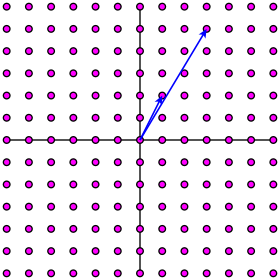
\includegraphics{Lattice_2}}
\caption{The lattice $\mathcal{L}(S_2)$.}
\label{F:Lattice_2}
\end{center}
\end{figure}


\ea

\end{pactivity}

Project Activity \ref{act:lattices_1} shows that even if $\CB$ is a basis for $\R^n$, it does not follow that $\mathcal{L}(\CB)$ is all of $\Z^n$. So latices can be complicated, and problems in lattice theory can be very difficult. 

The GGH cryptosystem relies on the fact that we can convert ``good" bases for lattices into ``bad" bases. We will not delve into the details of what separates a ``good" basis from a ``bad" one, but suffice it to say that a good basis is one in which the basis vectors are close to being perpendicular\footnote{This is also a good property in vector spaces. We will see in a later section that perpendicular basis vectors make calculations in vector spaces relatively easy. A similar thing is true in lattices, where we are able to solve certain variants of closest vector problem very efficiently.} and are all short (that is, they have small norms), while any other basis is a bad basis. An example of a good basis is the basis $S_1$ for $\R^2$ in Project Activity \ref{act:lattices_1}, and we will see later that $\{[-2 \ 8]^{\tr}, [-1 \ 3]^{\tr}\}$ is a bad basis for the same lattice. You should draw a picture of the vectors $[-2 \ 8]^{\tr}$ and $[-1 \ 3]^{\tr}$ to convince yourself that this is a bad basis for its lattice.  

The GGH cryptosystem works with two \emph{keys} -- a public key and a private key. The keys are based on lattices. The general process of the GGH cryptosystem is as follows. Begin with a good basis $\CB = \{\vb_1 \ \vb_2 \ \ldots \ \vb_n\}$ of $\R^n$ of vectors with integer components. Let $B = [\vb_1 \ \vb_2 \ \cdots \ \vb_n]$ be the matrix associated with $\CB$. Let $\CB' = \{\vb'_1, \vb'_2, \ldots, \vb'_n\}$ be a bad basis for which $\mathcal{L}(\CB') = \mathcal{L}(\CB)$. Let $B' = [\vb'_1 \ \vb'_2 \ \cdots \ \vb'_n]$ be the matrix associated to the basis $\CB'$. The bad basis can be shared with anyone (the public key), but the good basis is kept secret (the private key). Start with a message $\vm = [m_1 \ m_2 \ \cdots \ m_n]^{\tr}$ with integer entries to send. 

First we encrypt the message, which can be done by anyone who has the public key $\CB'$.
\begin{itemize}
\item Create the message vector 
\[\vm' = m_1 \vb'_1 +  m_2 \vb'_2 + \cdots +  m_n \vb'_n = B' \vm\]
that is in the lattice using the bad basis $\CB'$.
\item Choose a small error $\ve$ to add to $\vm'$ to move $\vm'$ off the lattice (small enough so that $\vm'$ does not pass by another lattice point). This is an important step that will make the message difficult to decrypt without the key. Let $\vc = \vm' + \ve = B'\vm + \ve$. The vector $\vc$ is the ciphertext that is to be transmitted to the receiver.
\end{itemize}

Only someone who knows the basis $\CB$ can decode the ciphertext. This is done as follows.
\begin{itemize}
\item Find the vector $\va = a_1 \vb_1 + a_2 \vb_2 + \cdots + a_n \vb_n$ in the good basis $\CB$ that is closest to $\vc$. 
\item We interpret the vector $[a_1 \ a_2 \ \ldots \ a_n]^{\tr}$ as being the encoded vector without the error. So to recreate the original message vector we need to undo the encrypting using the bad basis $\CB'$. That is, we need to find the weights $y_1$, $y_2$, $\ldots$, $y_n$ such that 
\[[a_1 \ a_2 \ \ldots \ a_n]^{\tr} = y_1 \vb'_1 + y_2 \vb'_2 + \cdots + y_n \vb'_n = B' [y_1 \ y_2 \ \cdots \ y_n]^{\tr}.\]
We can do this by as $[y_1 \ y_2 \ \cdots \ y_n]^{\tr} = B'^{-1} [a_1 \ a_2 \ \ldots \ a_n]^{\tr}$.
\end{itemize}

There are several items to address before we can implement this algorithm. One is how we create a bad basis $\CB'$ from $\CB$ that produces the same lattice. Another is how we find the vector in $\mathcal{\CB}$ closest to a given vector. The latter problem is called the Closest Vector Problem (CVP) and is, in general, a very difficult problem. This is what makes lattice-based cryptosystems secure. We address the first of these items in the next activity, and the second a bit later. 

 
\begin{pactivity} \label{act:lattices_2} Consider again the basis $S_1 = \{[1 \ 1]^{\tr}, [-1 \ 1]^{\tr}\}$ from Project Activity \ref{act:lattices_1}, and let $B = \left[ \begin{array}{cr} 1&-1\\1&1 \end{array} \right]$ be the matrix whose columns are the vectors in $S_1$. 
\ba
\item Let $T$ be the triangle with vertices $(0,0)$, $(1,1)$, and $(-1,1)$. Show that this triangle is a right triangle, and conclude that the vectors $\vv_1 = [1 \ 1]^{\tr}$, and $\vv_2 = [-1 \ 1]^{\tr}$ are perpendicular.


\item Let $U = \left[ \begin{array}{cc} 3&1\\5&2 \end{array} \right]$. Let $S_3$ be the set whose vectors are the columns of the matrix $B_1U$.  Show that $\mathcal{L}(S_1) = \mathcal{L}(S_3)$.

\ea

\end{pactivity}


The two bases $S_1 = \{[1 \ 1]^{\tr}, [-1 \ 1]^{\tr}\}$ and $S_3 =\{[-2 \ 8]^{\tr}, [-1 \ 3]^{\tr}\}$ from Project Activity \ref{act:lattices_2} are shown in Figure \ref{F:Lattice_3}. This figure illustrates how the matrix $U$ transforms the basis $S_1$, in which the vectors are perpendicular and short, to one in which the vectors are nearly parallel and significantly longer. So the matrix $U$ converts the ``good" basis $S_1$ into a ``bad" basis $S_2$, keeping the lattice intact. This is a key idea in the GGH cryptosystem. What makes this work is the fact that both $U$ and $U^{-1}$ have integer entries. The reason for this is that, for a $2 \times 2$ matrix $U = \left[ \begin{array}{cc} a&b\\c&d \end{array} \right]$, we know that $U^{-1} = \frac{1}{ad-bc} \left[  \begin{array}{rr} d&-b\\-c&a \end{array} \right]$. If $U$ has integer entries and $ad-bc = \pm 1$, then $U^{-1}$ will also have integer entries. The number $ad-bc$ is called the \emph{determinant} of $U$, and matrices with determinant of $1$ or $-1$ are called \emph{unimodular}. That what happened in Project Activity \ref{act:lattices_2} happens in the general case is the focus of the next activity.
\begin{figure}[h]
\begin{center}
\resizebox{!}{2.0in}{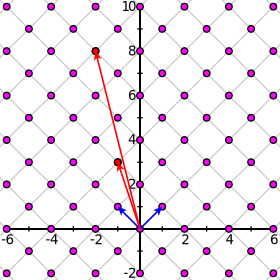
\includegraphics{Lattice_3}}
\caption{The lattices $\mathcal{L}(S_1)$ and $\mathcal{L}(S_3)$.}
\label{F:Lattice_3}
\end{center}
\end{figure}



\begin{pactivity} \label{act:lattices_3} We will restrict ourselves to $2 \times 2$ matrices in this activity, but the results generalize to $n \times n$ matrices. Let $\CB = \{\vb_1, \vb_2\}$ and $\CB' = \{\vb'_1, \vb'_2\}$ be bases for $\R^2$ with integer entries, and let $B = [\vb_1 \ \vb_2]$ and $B' = [\vb'_1 \ \vb'_2]$ be the matrices associated to these bases. Show that if $B' = BU$ for some unimodular matrix $U$ with integer entries, then $\mathcal{L}(B) = \mathcal{L}(B')$.


\end{pactivity}

Project Activity \ref{act:lattices_3} is the part we need for our lattice-based cryptosysystem. Although we won't show it here, the converse of the statement in Project Activity \ref{act:lattices_3} is also true. That is, if $\CB$ and $\CB'$ generate the same lattice, then $B' = BU$ for some unimodular matrix $U$ with integer entries.


There is one more item to address before we implement the GGH cryptosystem. That item is how to solve the Closest Vector Problem. There are some algorithms for approximating the closest vector in a basis. One is Babai's Closest Vector algorithm. This algorithm works in the following way. Consider a lattice with basis $\{\vb_1, \vb_2, \ldots, \vb_n\}$. To approximate the closest vector in the lattice to a vector $\vw$, find the weights $c_1$, $c_2$, $\ldots$, $c_n$ in $\R$ such that $\vw = c_1\vb_1 + c_2 \vb_2 + \cdots + c_n \vb_n$. Then round the coefficients to the nearest integer.  This algorithm works well for a good basis, but is unlikely to return a lattice point that is close to $\vw$ if the basis is a bad one. 

Now we put this all together to illustrate the GGH algorithm. 

\begin{figure}[h]
\begin{center}
\resizebox{!}{2.0in}{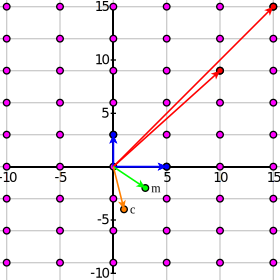
\includegraphics{GGH_example}}
\caption{Decrypting an encrypted message.}
\label{F:lattices_GGH_ex}
\end{center}
\end{figure}

\begin{pactivity} \label{act:lattices_GGH} Let $\CB = \{[5 \ 0]^{\tr}, [0 \ 3]^{\tr}\}$ be the private key, and let $B = \left[ \begin{array}{cc}5&0\\0&3 \end{array} \right]$ be the matrix whose columns are the vectors in $\CB$.  Let $U$ be the unimodular matrix $U = \left[ \begin{array}{cc} 2&3\\3&5 \end{array} \right]$. Let $\vm = [3 \ -2]^{\tr}$ be our message and let $\ve = [1 \ -1]^{\tr}$ be our error vector.
\ba
\item Use the unimodular matrix $U$ to create the bad basis $\CB'$. 

 
\item Determine the ciphertext message $\vc$.


\item A picture of the message vector $\vm$ and the ciphertext vector $\vc$ are shown in Figure \ref{F:lattices_GGH_ex}. Although the closest vector in the lattice to $\vc$ can be determined by the figure, actual messages are constructed in high dimensional spaces where a visual approach is not practical. Use Babai's algorithm to find the vector in $\mathcal{L}(\CB)$ that is closest to $\vc$ and compare to Figure \ref{F:lattices_GGH_ex}.


\item The final step in the GGH scheme is to recover the original message. Complete the GGH algorithm to find this message. 


\item The GGH cryptosystem works because the CVP can be reasonable solved using a good basis. That is, Babai's algorithm works if our basis is a good basis. To illustrate that a bad basis will not allow us to reproduce the original message vector, show that Babai's algorithm does not return the closest vector to $\vc$ using the bad basis $\CB'$.


\ea

\end{pactivity}

